\usubsection{Caso 2}

% \usubsubsection{Solución Teórica}
%
% \begin{align*}
%   R&=20k\Omega&
%   C&=100\mu F&
%   L&=7mH
% \end{align*}
% \begin{align*}
%   s_1 &= \frac{-\frac{20k\Omega}{7mH}
%   - \sqrt{\left(\frac{20k\Omega}{7mH}\right)^2-\frac{4}{7mH100\mu F}}}{2}
%   &
%   s_2 &= \frac{-\frac{20k\Omega}{7mH}
%   + \sqrt{\left(\frac{20k\Omega}{7mH}\right)^2-\frac{4}{7mH100\mu F}}}{2}
% \end{align*}

\usubsubsection{Simulación}

\begin{figure}[H]
  \lstinputlisting{modelica/RLCSerie2.mo}
  \caption{Código para el segundo caso.}
\end{figure}

\begin{figure}[H]
  \centering
  \label{gr:caso1:corrientes}
  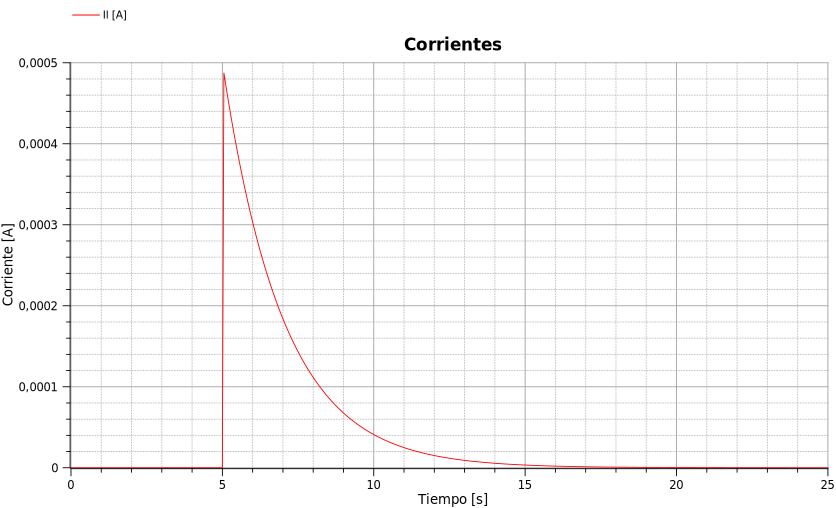
\includegraphics[width=\textwidth]{modelica/graficas/2-corrientes}
  \caption{Gráfica de Corrientes para el segundo caso.}
\end{figure}

\begin{figure}[H]
  \centering
  \label{gr:caso1:tensiones}
  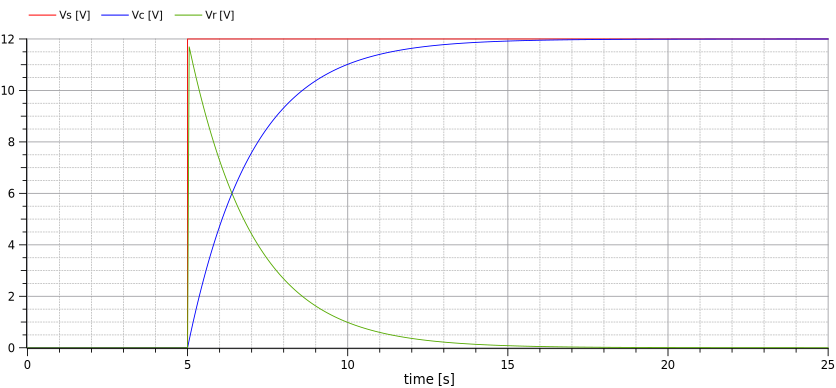
\includegraphics[width=\textwidth]{modelica/graficas/2-tensiones}
  \caption{Gráfica de Tensiones para el segundo caso.}
\end{figure}
